\section{mc\_\-constants.h File Reference}
\label{mc__constants_8h}\index{mc\_\-constants.h@{mc\_\-constants.h}}
{\tt \#include $<$math.h$>$}\par
{\tt \#include $<$stdint.h$>$}\par


Include dependency graph for mc\_\-constants.h:\nopagebreak
\begin{figure}[H]
\begin{center}
\leavevmode
\includegraphics[width=78pt]{mc__constants_8h__incl}
\end{center}
\end{figure}


This graph shows which files directly or indirectly include this file:\nopagebreak
\begin{figure}[H]
\begin{center}
\leavevmode
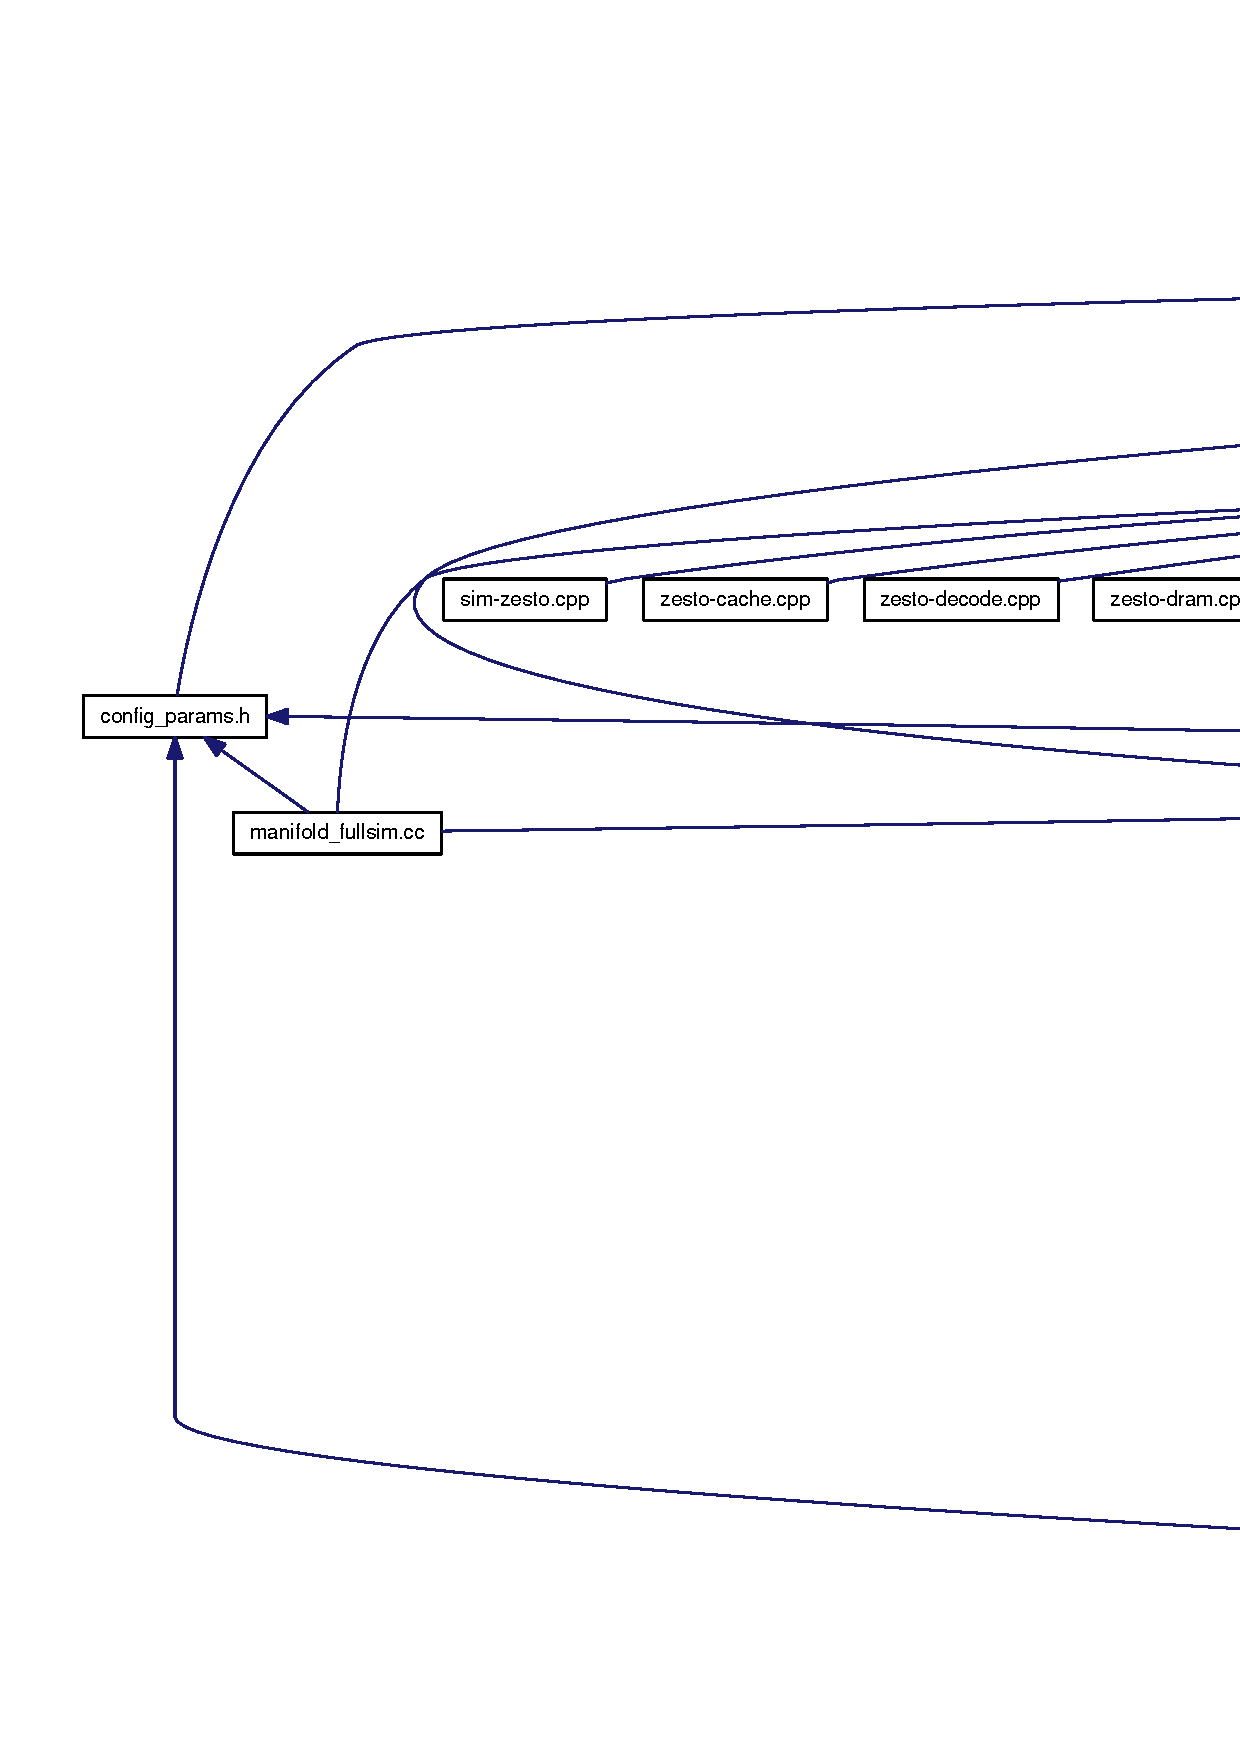
\includegraphics[width=420pt]{mc__constants_8h__dep__incl}
\end{center}
\end{figure}
\subsection*{Defines}
\begin{CompactItemize}
\item 
\#define {\bf DEBUG}
\item 
\#define {\bf DEEP\_\-DEBUG}
\item 
\#define {\bf NO\_\-OF\_\-CHANNELS}~1
\item 
\#define {\bf NO\_\-OF\_\-BUFFERS}~{\bf NO\_\-OF\_\-BANKS}
\item 
\#define {\bf BLOCKS\_\-PER\_\-ROW}~128
\item 
\#define {\bf CACHE\_\-BLOCK\_\-SIZE}~64
\item 
\#define {\bf ROW\_\-SIZE}~{\bf NO\_\-OF\_\-COLUMNS}$\ast${\bf COLUMN\_\-SIZE}
\item 
\#define {\bf DRAM\_\-SIZE}~{\bf NO\_\-OF\_\-CHANNELS}$\ast${\bf NO\_\-OF\_\-RANKS}$\ast${\bf NO\_\-OF\_\-BANKS}$\ast${\bf NO\_\-OF\_\-ROWS}$\ast${\bf ROW\_\-SIZE}
\item 
\#define {\bf TAG\_\-BITS}~8
\item 
\#define {\bf USE\_\-MSHR}~1
\item 
\#define {\bf BATCH\_\-FORM\_\-TIME}~2000;
\item 
\#define {\bf MAX\_\-BATCH\_\-SIZE}~5
\item 
\#define {\bf MAX\_\-READ\_\-OV\_\-WRITE}~8
\item 
\#define {\bf READ\_\-SIZE}~{\bf CACHE\_\-BLOCK\_\-SIZE}
\item 
\#define {\bf WRITE\_\-SIZE}~{\bf CACHE\_\-BLOCK\_\-SIZE}
\item 
\#define {\bf PREFETCH\_\-SIZE}~{\bf CACHE\_\-BLOCK\_\-SIZE}
\item 
\#define {\bf WRITEBACK\_\-SIZE}~{\bf CACHE\_\-BLOCK\_\-SIZE}
\item 
\#define {\bf REFRESH\_\-PERIOD}~{\bf CORE\_\-SPEED}$\ast$64000
\item 
\#define {\bf REFRESH\_\-INC}~({\bf ullint})floor({\bf REFRESH\_\-PERIOD}/(8192)) - {\bf BUS\_\-CYCLE}
\end{CompactItemize}
\subsection*{Typedefs}
\begin{CompactItemize}
\item 
typedef unsigned long long int {\bf Time}
\item 
typedef unsigned long long int {\bf Addr\_\-t}
\item 
typedef unsigned int {\bf uint}
\item 
typedef unsigned int {\bf UInt}
\end{CompactItemize}
\subsection*{Enumerations}
\begin{CompactItemize}
\item 
enum {\bf DRAM\_\-PAGE\_\-POLICY} \{ {\bf OPEN\_\-PAGE\_\-POLICY}, 
{\bf CLOSE\_\-PAGE\_\-POLICY}, 
{\bf OPEN\_\-PAGE\_\-POLICY}, 
{\bf CLOSE\_\-PAGE\_\-POLICY}
 \}
\item 
enum {\bf MC\_\-SCHEDULLING\_\-ALGO} \{ \par
{\bf PAR\_\-BS}, 
{\bf FR\_\-FCFS}, 
{\bf FC\_\-FS}, 
{\bf NFQ}, 
\par
{\bf PAR\_\-BS}, 
{\bf FR\_\-FCFS}, 
{\bf FC\_\-FS}, 
{\bf NFQ}
 \}
\item 
enum {\bf ADDR\_\-MAP\_\-SCHEME} \{ \par
{\bf PAGE\_\-INTERLEAVING}, 
{\bf PERMUTATION}, 
{\bf CACHELINE\_\-INTERLEAVING}, 
{\bf SWAPPING}, 
\par
{\bf GENERIC}, 
{\bf NO\_\-SCHEME}, 
{\bf LOCAL\_\-ADDR\_\-MAP}, 
{\bf PAGE\_\-INTERLEAVING}, 
\par
{\bf PERMUTATION}, 
{\bf CACHELINE\_\-INTERLEAVING}, 
{\bf SWAPPING}, 
{\bf GENERIC}, 
\par
{\bf NO\_\-SCHEME}, 
{\bf LOCAL\_\-ADDR\_\-MAP}
 \}
\item 
enum {\bf DRAM\_\-CONFIG} \{ \par
{\bf DDR3\_\-1333\_\-9\_\-9\_\-9}, 
{\bf DDR3\_\-1600\_\-10\_\-10\_\-10}, 
{\bf DDR3\_\-1333\_\-6\_\-6\_\-6}, 
{\bf DDR2\_\-533\_\-4\_\-4\_\-4}, 
\par
{\bf DDR2\_\-667\_\-4\_\-4\_\-4}, 
{\bf DDR3\_\-1333\_\-9}, 
{\bf DDR3\_\-1600\_\-10}, 
{\bf DDR3\_\-1333\_\-6}, 
\par
{\bf DDR2\_\-533\_\-4}, 
{\bf DDR2\_\-667\_\-4}
 \}
\end{CompactItemize}
\subsection*{Variables}
\begin{CompactItemize}
\item 
{\bf DRAM\_\-PAGE\_\-POLICY} {\bf dram\_\-page\_\-policy}
\item 
{\bf MC\_\-SCHEDULLING\_\-ALGO} {\bf mc\_\-scheduling\_\-algorithm}
\item 
{\bf ADDR\_\-MAP\_\-SCHEME} {\bf addr\_\-map\_\-scheme}
\item 
{\bf uint} {\bf NO\_\-OF\_\-THREADS}
\item 
{\bf uint} {\bf NO\_\-OF\_\-RANKS}
\item 
{\bf uint} {\bf NO\_\-OF\_\-BANKS}
\item 
{\bf uint} {\bf NO\_\-OF\_\-ROWS}
\item 
{\bf uint} {\bf NO\_\-OF\_\-COLUMNS}
\item 
{\bf uint} {\bf COLUMN\_\-SIZE}
\item 
{\bf uint} {\bf MSHR\_\-SIZE}
\item 
{\bf uint} {\bf MAX\_\-BUFFER\_\-SIZE}
\item 
{\bf uint} {\bf MAX\_\-CMD\_\-BUFFER\_\-SIZE}
\item 
{\bf uint} {\bf RESPONSE\_\-BUFFER\_\-SIZE}
\item 
{\bf uint} {\bf NETWORK\_\-ADDRESS\_\-BITS}
\item 
{\bf uint} {\bf NETWORK\_\-THREADID\_\-BITS}
\item 
{\bf uint} {\bf NETWORK\_\-COMMAND\_\-BITS}
\item 
float {\bf CORE\_\-SPEED}
\item 
float {\bf CYCLE\_\-2\_\-NS}
\item 
unsigned int {\bf DDR\_\-BUS\_\-WIDTH}
\item 
float {\bf BUS\_\-SPEED}
\item 
float {\bf MEM\_\-SPEED}
\item 
float {\bf MEM\_\-CYCLE}
\item 
float {\bf BUS\_\-CYCLE}
\item 
float {\bf tREFI}
\item 
float {\bf tRFC}
\item 
float {\bf tRC}
\item 
float {\bf tRAS}
\item 
unsigned int {\bf t\_\-CMD}
\item 
unsigned int {\bf t\_\-RCD}
\item 
unsigned int {\bf t\_\-RRD}
\item 
unsigned int {\bf t\_\-RAS}
\item 
unsigned int {\bf t\_\-CAS}
\item 
unsigned int {\bf t\_\-RTRS}
\item 
unsigned int {\bf t\_\-OST}
\item 
unsigned int {\bf t\_\-WR}
\item 
unsigned int {\bf t\_\-WTR}
\item 
unsigned int {\bf t\_\-RP}
\item 
unsigned int {\bf t\_\-CCD}
\item 
unsigned int {\bf t\_\-AL}
\item 
unsigned int {\bf t\_\-CWD}
\item 
unsigned int {\bf t\_\-RC}
\item 
unsigned int {\bf t\_\-RTP}
\item 
unsigned int {\bf t\_\-RFC}
\end{CompactItemize}


\subsection{Define Documentation}
\index{mc\_\-constants.h@{mc\_\-constants.h}!BATCH\_\-FORM\_\-TIME@{BATCH\_\-FORM\_\-TIME}}
\index{BATCH\_\-FORM\_\-TIME@{BATCH\_\-FORM\_\-TIME}!mc_constants.h@{mc\_\-constants.h}}
\subsubsection[{BATCH\_\-FORM\_\-TIME}]{\setlength{\rightskip}{0pt plus 5cm}\#define {\bf BATCH\_\-FORM\_\-TIME}~2000;}\label{mc__constants_8h_e7e3459c7023f3a7dcd68b382db8da3d}




Definition at line 74 of file mc\_\-constants.h.

Referenced by RequestHandler::FormBatch(), and RequestHandler::process\_\-event().\index{mc\_\-constants.h@{mc\_\-constants.h}!BLOCKS\_\-PER\_\-ROW@{BLOCKS\_\-PER\_\-ROW}}
\index{BLOCKS\_\-PER\_\-ROW@{BLOCKS\_\-PER\_\-ROW}!mc_constants.h@{mc\_\-constants.h}}
\subsubsection[{BLOCKS\_\-PER\_\-ROW}]{\setlength{\rightskip}{0pt plus 5cm}\#define {\bf BLOCKS\_\-PER\_\-ROW}~128}\label{mc__constants_8h_049e7586f4dee8bf82b0db100e1c36d4}




Definition at line 60 of file mc\_\-constants.h.

Referenced by MSHR\_\-H::local\_\-map\_\-addr(), and AddrMap::map\_\-addr().\index{mc\_\-constants.h@{mc\_\-constants.h}!CACHE\_\-BLOCK\_\-SIZE@{CACHE\_\-BLOCK\_\-SIZE}}
\index{CACHE\_\-BLOCK\_\-SIZE@{CACHE\_\-BLOCK\_\-SIZE}!mc_constants.h@{mc\_\-constants.h}}
\subsubsection[{CACHE\_\-BLOCK\_\-SIZE}]{\setlength{\rightskip}{0pt plus 5cm}\#define {\bf CACHE\_\-BLOCK\_\-SIZE}~64}\label{mc__constants_8h_9e92828e1e7a7cc03003c00282384f96}




Definition at line 61 of file mc\_\-constants.h.

Referenced by uncore\_\-t::convertFromBitStream(), GenericTPGVcs::convertFromBitStream(), GenericTPG::convertFromBitStream(), uncore\_\-t::convertToBitStream(), NI::convertToBitStream(), GenericTPGVcs::convertToBitStream(), GenericTPG::convertToBitStream(), MSHR\_\-H::local\_\-map\_\-addr(), and AddrMap::map\_\-addr().\index{mc\_\-constants.h@{mc\_\-constants.h}!DEBUG@{DEBUG}}
\index{DEBUG@{DEBUG}!mc_constants.h@{mc\_\-constants.h}}
\subsubsection[{DEBUG}]{\setlength{\rightskip}{0pt plus 5cm}\#define DEBUG}\label{mc__constants_8h_d72dbcf6d0153db1b8d8a58001feed83}




Definition at line 23 of file mc\_\-constants.h.

Referenced by GenericTPGVcs::handle\_\-new\_\-packet\_\-event().\index{mc\_\-constants.h@{mc\_\-constants.h}!DEEP\_\-DEBUG@{DEEP\_\-DEBUG}}
\index{DEEP\_\-DEBUG@{DEEP\_\-DEBUG}!mc_constants.h@{mc\_\-constants.h}}
\subsubsection[{DEEP\_\-DEBUG}]{\setlength{\rightskip}{0pt plus 5cm}\#define DEEP\_\-DEBUG}\label{mc__constants_8h_98846f5e42d3145d826f8b664ec13f80}




Definition at line 24 of file mc\_\-constants.h.\index{mc\_\-constants.h@{mc\_\-constants.h}!DRAM\_\-SIZE@{DRAM\_\-SIZE}}
\index{DRAM\_\-SIZE@{DRAM\_\-SIZE}!mc_constants.h@{mc\_\-constants.h}}
\subsubsection[{DRAM\_\-SIZE}]{\setlength{\rightskip}{0pt plus 5cm}\#define {\bf DRAM\_\-SIZE}~{\bf NO\_\-OF\_\-CHANNELS}$\ast${\bf NO\_\-OF\_\-RANKS}$\ast${\bf NO\_\-OF\_\-BANKS}$\ast${\bf NO\_\-OF\_\-ROWS}$\ast${\bf ROW\_\-SIZE}}\label{mc__constants_8h_4e35909b44ea391fbb7bb146992bb84d}




Definition at line 63 of file mc\_\-constants.h.

Referenced by MSHR\_\-H::local\_\-map\_\-addr(), and AddrMap::map\_\-addr().\index{mc\_\-constants.h@{mc\_\-constants.h}!MAX\_\-BATCH\_\-SIZE@{MAX\_\-BATCH\_\-SIZE}}
\index{MAX\_\-BATCH\_\-SIZE@{MAX\_\-BATCH\_\-SIZE}!mc_constants.h@{mc\_\-constants.h}}
\subsubsection[{MAX\_\-BATCH\_\-SIZE}]{\setlength{\rightskip}{0pt plus 5cm}\#define {\bf MAX\_\-BATCH\_\-SIZE}~5}\label{mc__constants_8h_18373cd65e0761a3bd4e760a8e015baa}




Definition at line 75 of file mc\_\-constants.h.

Referenced by RequestHandler::MarkBatchOnly().\index{mc\_\-constants.h@{mc\_\-constants.h}!MAX\_\-READ\_\-OV\_\-WRITE@{MAX\_\-READ\_\-OV\_\-WRITE}}
\index{MAX\_\-READ\_\-OV\_\-WRITE@{MAX\_\-READ\_\-OV\_\-WRITE}!mc_constants.h@{mc\_\-constants.h}}
\subsubsection[{MAX\_\-READ\_\-OV\_\-WRITE}]{\setlength{\rightskip}{0pt plus 5cm}\#define {\bf MAX\_\-READ\_\-OV\_\-WRITE}~8}\label{mc__constants_8h_807dcc509b3155f4be5d3979e3d910dd}




Definition at line 76 of file mc\_\-constants.h.

Referenced by BankHandler::ReadsFirst().\index{mc\_\-constants.h@{mc\_\-constants.h}!NO\_\-OF\_\-BUFFERS@{NO\_\-OF\_\-BUFFERS}}
\index{NO\_\-OF\_\-BUFFERS@{NO\_\-OF\_\-BUFFERS}!mc_constants.h@{mc\_\-constants.h}}
\subsubsection[{NO\_\-OF\_\-BUFFERS}]{\setlength{\rightskip}{0pt plus 5cm}\#define {\bf NO\_\-OF\_\-BUFFERS}~{\bf NO\_\-OF\_\-BANKS}}\label{mc__constants_8h_a9f2d328954a62b047317e13f33bda12}




Definition at line 56 of file mc\_\-constants.h.

Referenced by Statistic::CollectStatsPerCycle(), GenericTPG::convertFromBitStream(), BankHandler::FindHighest(), Statistic::InitStats(), RequestHandler::MarkAll(), RequestHandler::MarkBatchOnly(), Statistic::PrintAggregateStats(), and RequestHandler::RequestHandler().\index{mc\_\-constants.h@{mc\_\-constants.h}!NO\_\-OF\_\-CHANNELS@{NO\_\-OF\_\-CHANNELS}}
\index{NO\_\-OF\_\-CHANNELS@{NO\_\-OF\_\-CHANNELS}!mc_constants.h@{mc\_\-constants.h}}
\subsubsection[{NO\_\-OF\_\-CHANNELS}]{\setlength{\rightskip}{0pt plus 5cm}\#define {\bf NO\_\-OF\_\-CHANNELS}~1}\label{mc__constants_8h_c60f68d55e472737b2890684e0d41ab9}




Definition at line 53 of file mc\_\-constants.h.

Referenced by BusHandler::BusHandler(), Statistic::CalculateAggregateStats(), Statistic::CollectStatsPerCycle(), DRAM::DRAM(), Statistic::InitStats(), MSHR\_\-H::local\_\-map\_\-addr(), BusHandler::LowLevelCmdGen(), AddrMap::map\_\-addr(), RequestHandler::MarkAll(), RequestHandler::MarkBatchOnly(), Statistic::PrintAggregateStats(), RequestHandler::process\_\-event(), RefreshMgr::process\_\-event(), Request::Request(), RequestHandler::RequestHandler(), BusHandler::SetIfFull(), RequestHandler::SetLinks(), DRAM::SetLinks(), and Bus::SetLinks().\index{mc\_\-constants.h@{mc\_\-constants.h}!PREFETCH\_\-SIZE@{PREFETCH\_\-SIZE}}
\index{PREFETCH\_\-SIZE@{PREFETCH\_\-SIZE}!mc_constants.h@{mc\_\-constants.h}}
\subsubsection[{PREFETCH\_\-SIZE}]{\setlength{\rightskip}{0pt plus 5cm}\#define {\bf PREFETCH\_\-SIZE}~{\bf CACHE\_\-BLOCK\_\-SIZE}}\label{mc__constants_8h_9c2cf5515858ee2f97a157ca23de784f}




Definition at line 84 of file mc\_\-constants.h.

Referenced by CmdIssuer::CalculateBurstL(), and DRAMCmdState::set().\index{mc\_\-constants.h@{mc\_\-constants.h}!READ\_\-SIZE@{READ\_\-SIZE}}
\index{READ\_\-SIZE@{READ\_\-SIZE}!mc_constants.h@{mc\_\-constants.h}}
\subsubsection[{READ\_\-SIZE}]{\setlength{\rightskip}{0pt plus 5cm}\#define {\bf READ\_\-SIZE}~{\bf CACHE\_\-BLOCK\_\-SIZE}}\label{mc__constants_8h_86e1969b50e55e5d506233078ca0fa4c}




Definition at line 82 of file mc\_\-constants.h.

Referenced by CmdIssuer::CalculateBurstL(), and DRAMCmdState::set().\index{mc\_\-constants.h@{mc\_\-constants.h}!REFRESH\_\-INC@{REFRESH\_\-INC}}
\index{REFRESH\_\-INC@{REFRESH\_\-INC}!mc_constants.h@{mc\_\-constants.h}}
\subsubsection[{REFRESH\_\-INC}]{\setlength{\rightskip}{0pt plus 5cm}\#define {\bf REFRESH\_\-INC}~({\bf ullint})floor({\bf REFRESH\_\-PERIOD}/(8192)) - {\bf BUS\_\-CYCLE}}\label{mc__constants_8h_aebf6da1474d52a416fbf00608e500cd}




Definition at line 88 of file mc\_\-constants.h.

Referenced by RefreshMgr::process\_\-event(), and MC::StartRefresh().\index{mc\_\-constants.h@{mc\_\-constants.h}!REFRESH\_\-PERIOD@{REFRESH\_\-PERIOD}}
\index{REFRESH\_\-PERIOD@{REFRESH\_\-PERIOD}!mc_constants.h@{mc\_\-constants.h}}
\subsubsection[{REFRESH\_\-PERIOD}]{\setlength{\rightskip}{0pt plus 5cm}\#define {\bf REFRESH\_\-PERIOD}~{\bf CORE\_\-SPEED}$\ast$64000}\label{mc__constants_8h_4ca70e92b8b779d01eed94f5f07a03ed}




Definition at line 87 of file mc\_\-constants.h.\index{mc\_\-constants.h@{mc\_\-constants.h}!ROW\_\-SIZE@{ROW\_\-SIZE}}
\index{ROW\_\-SIZE@{ROW\_\-SIZE}!mc_constants.h@{mc\_\-constants.h}}
\subsubsection[{ROW\_\-SIZE}]{\setlength{\rightskip}{0pt plus 5cm}\#define {\bf ROW\_\-SIZE}~{\bf NO\_\-OF\_\-COLUMNS}$\ast${\bf COLUMN\_\-SIZE}}\label{mc__constants_8h_a4d030604a90c8d019d90fc721900d63}




Definition at line 62 of file mc\_\-constants.h.

Referenced by MSHR\_\-H::local\_\-map\_\-addr(), AddrMap::map\_\-addr(), and RefreshMgr::process\_\-event().\index{mc\_\-constants.h@{mc\_\-constants.h}!TAG\_\-BITS@{TAG\_\-BITS}}
\index{TAG\_\-BITS@{TAG\_\-BITS}!mc_constants.h@{mc\_\-constants.h}}
\subsubsection[{TAG\_\-BITS}]{\setlength{\rightskip}{0pt plus 5cm}\#define {\bf TAG\_\-BITS}~8}\label{mc__constants_8h_273bfff4ad6c875e1d4ca56b70a23137}




Definition at line 64 of file mc\_\-constants.h.

Referenced by MSHR\_\-H::local\_\-map\_\-addr(), and AddrMap::map\_\-addr().\index{mc\_\-constants.h@{mc\_\-constants.h}!USE\_\-MSHR@{USE\_\-MSHR}}
\index{USE\_\-MSHR@{USE\_\-MSHR}!mc_constants.h@{mc\_\-constants.h}}
\subsubsection[{USE\_\-MSHR}]{\setlength{\rightskip}{0pt plus 5cm}\#define {\bf USE\_\-MSHR}~1}\label{mc__constants_8h_6021de24ebedf19345f1d5a34fc92c22}




Definition at line 66 of file mc\_\-constants.h.\index{mc\_\-constants.h@{mc\_\-constants.h}!WRITE\_\-SIZE@{WRITE\_\-SIZE}}
\index{WRITE\_\-SIZE@{WRITE\_\-SIZE}!mc_constants.h@{mc\_\-constants.h}}
\subsubsection[{WRITE\_\-SIZE}]{\setlength{\rightskip}{0pt plus 5cm}\#define {\bf WRITE\_\-SIZE}~{\bf CACHE\_\-BLOCK\_\-SIZE}}\label{mc__constants_8h_dffc7bcd50015cae98ad6b1f3e240c03}




Definition at line 83 of file mc\_\-constants.h.

Referenced by CmdIssuer::CalculateBurstL(), and DRAMCmdState::set().\index{mc\_\-constants.h@{mc\_\-constants.h}!WRITEBACK\_\-SIZE@{WRITEBACK\_\-SIZE}}
\index{WRITEBACK\_\-SIZE@{WRITEBACK\_\-SIZE}!mc_constants.h@{mc\_\-constants.h}}
\subsubsection[{WRITEBACK\_\-SIZE}]{\setlength{\rightskip}{0pt plus 5cm}\#define {\bf WRITEBACK\_\-SIZE}~{\bf CACHE\_\-BLOCK\_\-SIZE}}\label{mc__constants_8h_9117e1b8ef1ac1f3fea5da3f3b883c9d}




Definition at line 85 of file mc\_\-constants.h.

Referenced by CmdIssuer::CalculateBurstL(), and DRAMCmdState::set().

\subsection{Typedef Documentation}
\index{mc\_\-constants.h@{mc\_\-constants.h}!Addr\_\-t@{Addr\_\-t}}
\index{Addr\_\-t@{Addr\_\-t}!mc_constants.h@{mc\_\-constants.h}}
\subsubsection[{Addr\_\-t}]{\setlength{\rightskip}{0pt plus 5cm}typedef unsigned long long int {\bf Addr\_\-t}}\label{mc__constants_8h_51badf0ffa6471a1e529c69852e56f57}




Definition at line 27 of file mc\_\-constants.h.\index{mc\_\-constants.h@{mc\_\-constants.h}!Time@{Time}}
\index{Time@{Time}!mc_constants.h@{mc\_\-constants.h}}
\subsubsection[{Time}]{\setlength{\rightskip}{0pt plus 5cm}typedef unsigned long long int {\bf Time}}\label{mc__constants_8h_a475e5c84e5eb0fe317942dc62553f7e}




Definition at line 26 of file mc\_\-constants.h.\index{mc\_\-constants.h@{mc\_\-constants.h}!UInt@{UInt}}
\index{UInt@{UInt}!mc_constants.h@{mc\_\-constants.h}}
\subsubsection[{UInt}]{\setlength{\rightskip}{0pt plus 5cm}typedef unsigned int {\bf UInt}}\label{mc__constants_8h_ba0996d26f7be2572973245b51852757}




Definition at line 29 of file mc\_\-constants.h.\index{mc\_\-constants.h@{mc\_\-constants.h}!uint@{uint}}
\index{uint@{uint}!mc_constants.h@{mc\_\-constants.h}}
\subsubsection[{uint}]{\setlength{\rightskip}{0pt plus 5cm}typedef unsigned int {\bf uint}}\label{mc__constants_8h_91ad9478d81a7aaf2593e8d9c3d06a14}




Definition at line 28 of file mc\_\-constants.h.

\subsection{Enumeration Type Documentation}
\index{mc\_\-constants.h@{mc\_\-constants.h}!ADDR\_\-MAP\_\-SCHEME@{ADDR\_\-MAP\_\-SCHEME}}
\index{ADDR\_\-MAP\_\-SCHEME@{ADDR\_\-MAP\_\-SCHEME}!mc_constants.h@{mc\_\-constants.h}}
\subsubsection[{ADDR\_\-MAP\_\-SCHEME}]{\setlength{\rightskip}{0pt plus 5cm}enum {\bf ADDR\_\-MAP\_\-SCHEME}}\label{mc__constants_8h_5070e557d1fe0f8dfbfe47ffb8feb753}


\begin{Desc}
\item[Enumerator: ]\par
\begin{description}
\index{PAGE\_\-INTERLEAVING@{PAGE\_\-INTERLEAVING}!mc\_\-constants.h@{mc\_\-constants.h}}\index{mc\_\-constants.h@{mc\_\-constants.h}!PAGE\_\-INTERLEAVING@{PAGE\_\-INTERLEAVING}}\item[{\em 
PAGE\_\-INTERLEAVING\label{mc__constants_8h_5070e557d1fe0f8dfbfe47ffb8feb7536318d7b959b906483ab378e56405a7a0}
}]\index{PERMUTATION@{PERMUTATION}!mc\_\-constants.h@{mc\_\-constants.h}}\index{mc\_\-constants.h@{mc\_\-constants.h}!PERMUTATION@{PERMUTATION}}\item[{\em 
PERMUTATION\label{mc__constants_8h_5070e557d1fe0f8dfbfe47ffb8feb75391bebfe0b6592c69090ade437798b19b}
}]\index{CACHELINE\_\-INTERLEAVING@{CACHELINE\_\-INTERLEAVING}!mc\_\-constants.h@{mc\_\-constants.h}}\index{mc\_\-constants.h@{mc\_\-constants.h}!CACHELINE\_\-INTERLEAVING@{CACHELINE\_\-INTERLEAVING}}\item[{\em 
CACHELINE\_\-INTERLEAVING\label{mc__constants_8h_5070e557d1fe0f8dfbfe47ffb8feb75314219aa18138d58f46b69b57e01efbeb}
}]\index{SWAPPING@{SWAPPING}!mc\_\-constants.h@{mc\_\-constants.h}}\index{mc\_\-constants.h@{mc\_\-constants.h}!SWAPPING@{SWAPPING}}\item[{\em 
SWAPPING\label{mc__constants_8h_5070e557d1fe0f8dfbfe47ffb8feb7530ce3016e7d4844b6546c795caf020ef1}
}]\index{GENERIC@{GENERIC}!mc\_\-constants.h@{mc\_\-constants.h}}\index{mc\_\-constants.h@{mc\_\-constants.h}!GENERIC@{GENERIC}}\item[{\em 
GENERIC\label{mc__constants_8h_5070e557d1fe0f8dfbfe47ffb8feb7539e022e6380da28dd73210ed34b137c36}
}]\index{NO\_\-SCHEME@{NO\_\-SCHEME}!mc\_\-constants.h@{mc\_\-constants.h}}\index{mc\_\-constants.h@{mc\_\-constants.h}!NO\_\-SCHEME@{NO\_\-SCHEME}}\item[{\em 
NO\_\-SCHEME\label{mc__constants_8h_5070e557d1fe0f8dfbfe47ffb8feb753ccb106f572e6684c377552afac75dac9}
}]\index{LOCAL\_\-ADDR\_\-MAP@{LOCAL\_\-ADDR\_\-MAP}!mc\_\-constants.h@{mc\_\-constants.h}}\index{mc\_\-constants.h@{mc\_\-constants.h}!LOCAL\_\-ADDR\_\-MAP@{LOCAL\_\-ADDR\_\-MAP}}\item[{\em 
LOCAL\_\-ADDR\_\-MAP\label{mc__constants_8h_5070e557d1fe0f8dfbfe47ffb8feb753705c391e0d76021b61cd7e74c72e1a64}
}]\index{PAGE\_\-INTERLEAVING@{PAGE\_\-INTERLEAVING}!mc\_\-constants.h@{mc\_\-constants.h}}\index{mc\_\-constants.h@{mc\_\-constants.h}!PAGE\_\-INTERLEAVING@{PAGE\_\-INTERLEAVING}}\item[{\em 
PAGE\_\-INTERLEAVING\label{mc__constants_8h_5070e557d1fe0f8dfbfe47ffb8feb7536318d7b959b906483ab378e56405a7a0}
}]\index{PERMUTATION@{PERMUTATION}!mc\_\-constants.h@{mc\_\-constants.h}}\index{mc\_\-constants.h@{mc\_\-constants.h}!PERMUTATION@{PERMUTATION}}\item[{\em 
PERMUTATION\label{mc__constants_8h_5070e557d1fe0f8dfbfe47ffb8feb75391bebfe0b6592c69090ade437798b19b}
}]\index{CACHELINE\_\-INTERLEAVING@{CACHELINE\_\-INTERLEAVING}!mc\_\-constants.h@{mc\_\-constants.h}}\index{mc\_\-constants.h@{mc\_\-constants.h}!CACHELINE\_\-INTERLEAVING@{CACHELINE\_\-INTERLEAVING}}\item[{\em 
CACHELINE\_\-INTERLEAVING\label{mc__constants_8h_5070e557d1fe0f8dfbfe47ffb8feb75314219aa18138d58f46b69b57e01efbeb}
}]\index{SWAPPING@{SWAPPING}!mc\_\-constants.h@{mc\_\-constants.h}}\index{mc\_\-constants.h@{mc\_\-constants.h}!SWAPPING@{SWAPPING}}\item[{\em 
SWAPPING\label{mc__constants_8h_5070e557d1fe0f8dfbfe47ffb8feb7530ce3016e7d4844b6546c795caf020ef1}
}]\index{GENERIC@{GENERIC}!mc\_\-constants.h@{mc\_\-constants.h}}\index{mc\_\-constants.h@{mc\_\-constants.h}!GENERIC@{GENERIC}}\item[{\em 
GENERIC\label{mc__constants_8h_5070e557d1fe0f8dfbfe47ffb8feb7539e022e6380da28dd73210ed34b137c36}
}]\index{NO\_\-SCHEME@{NO\_\-SCHEME}!mc\_\-constants.h@{mc\_\-constants.h}}\index{mc\_\-constants.h@{mc\_\-constants.h}!NO\_\-SCHEME@{NO\_\-SCHEME}}\item[{\em 
NO\_\-SCHEME\label{mc__constants_8h_5070e557d1fe0f8dfbfe47ffb8feb753ccb106f572e6684c377552afac75dac9}
}]\index{LOCAL\_\-ADDR\_\-MAP@{LOCAL\_\-ADDR\_\-MAP}!mc\_\-constants.h@{mc\_\-constants.h}}\index{mc\_\-constants.h@{mc\_\-constants.h}!LOCAL\_\-ADDR\_\-MAP@{LOCAL\_\-ADDR\_\-MAP}}\item[{\em 
LOCAL\_\-ADDR\_\-MAP\label{mc__constants_8h_5070e557d1fe0f8dfbfe47ffb8feb753705c391e0d76021b61cd7e74c72e1a64}
}]\end{description}
\end{Desc}



Definition at line 41 of file mc\_\-constants.h.\index{mc\_\-constants.h@{mc\_\-constants.h}!DRAM\_\-CONFIG@{DRAM\_\-CONFIG}}
\index{DRAM\_\-CONFIG@{DRAM\_\-CONFIG}!mc_constants.h@{mc\_\-constants.h}}
\subsubsection[{DRAM\_\-CONFIG}]{\setlength{\rightskip}{0pt plus 5cm}enum {\bf DRAM\_\-CONFIG}}\label{mc__constants_8h_e9e4ff36044e2d5a86faa987c553bd3c}


\begin{Desc}
\item[Enumerator: ]\par
\begin{description}
\index{DDR3\_\-1333\_\-9\_\-9\_\-9@{DDR3\_\-1333\_\-9\_\-9\_\-9}!mc\_\-constants.h@{mc\_\-constants.h}}\index{mc\_\-constants.h@{mc\_\-constants.h}!DDR3\_\-1333\_\-9\_\-9\_\-9@{DDR3\_\-1333\_\-9\_\-9\_\-9}}\item[{\em 
DDR3\_\-1333\_\-9\_\-9\_\-9\label{mc__constants_8h_e9e4ff36044e2d5a86faa987c553bd3c712c348582ed4edfb090d8c73b8b5391}
}]\index{DDR3\_\-1600\_\-10\_\-10\_\-10@{DDR3\_\-1600\_\-10\_\-10\_\-10}!mc\_\-constants.h@{mc\_\-constants.h}}\index{mc\_\-constants.h@{mc\_\-constants.h}!DDR3\_\-1600\_\-10\_\-10\_\-10@{DDR3\_\-1600\_\-10\_\-10\_\-10}}\item[{\em 
DDR3\_\-1600\_\-10\_\-10\_\-10\label{mc__constants_8h_e9e4ff36044e2d5a86faa987c553bd3c12473400467619bf225c5f29af3799a2}
}]\index{DDR3\_\-1333\_\-6\_\-6\_\-6@{DDR3\_\-1333\_\-6\_\-6\_\-6}!mc\_\-constants.h@{mc\_\-constants.h}}\index{mc\_\-constants.h@{mc\_\-constants.h}!DDR3\_\-1333\_\-6\_\-6\_\-6@{DDR3\_\-1333\_\-6\_\-6\_\-6}}\item[{\em 
DDR3\_\-1333\_\-6\_\-6\_\-6\label{mc__constants_8h_e9e4ff36044e2d5a86faa987c553bd3c59e4aeb7c22ad8de2d7a59f51a38c699}
}]\index{DDR2\_\-533\_\-4\_\-4\_\-4@{DDR2\_\-533\_\-4\_\-4\_\-4}!mc\_\-constants.h@{mc\_\-constants.h}}\index{mc\_\-constants.h@{mc\_\-constants.h}!DDR2\_\-533\_\-4\_\-4\_\-4@{DDR2\_\-533\_\-4\_\-4\_\-4}}\item[{\em 
DDR2\_\-533\_\-4\_\-4\_\-4\label{mc__constants_8h_e9e4ff36044e2d5a86faa987c553bd3c0ff5eab57ec99b2f02cfbb355cf77234}
}]\index{DDR2\_\-667\_\-4\_\-4\_\-4@{DDR2\_\-667\_\-4\_\-4\_\-4}!mc\_\-constants.h@{mc\_\-constants.h}}\index{mc\_\-constants.h@{mc\_\-constants.h}!DDR2\_\-667\_\-4\_\-4\_\-4@{DDR2\_\-667\_\-4\_\-4\_\-4}}\item[{\em 
DDR2\_\-667\_\-4\_\-4\_\-4\label{mc__constants_8h_e9e4ff36044e2d5a86faa987c553bd3cee61db8fff3689314f94bfbd49817c46}
}]\index{DDR3\_\-1333\_\-9@{DDR3\_\-1333\_\-9}!mc\_\-constants.h@{mc\_\-constants.h}}\index{mc\_\-constants.h@{mc\_\-constants.h}!DDR3\_\-1333\_\-9@{DDR3\_\-1333\_\-9}}\item[{\em 
DDR3\_\-1333\_\-9\label{mc__constants_8h_e9e4ff36044e2d5a86faa987c553bd3cff807c763cb52ea99c781812686ea277}
}]\index{DDR3\_\-1600\_\-10@{DDR3\_\-1600\_\-10}!mc\_\-constants.h@{mc\_\-constants.h}}\index{mc\_\-constants.h@{mc\_\-constants.h}!DDR3\_\-1600\_\-10@{DDR3\_\-1600\_\-10}}\item[{\em 
DDR3\_\-1600\_\-10\label{mc__constants_8h_e9e4ff36044e2d5a86faa987c553bd3cea8ed17daab991b7c28b7f32cd25e884}
}]\index{DDR3\_\-1333\_\-6@{DDR3\_\-1333\_\-6}!mc\_\-constants.h@{mc\_\-constants.h}}\index{mc\_\-constants.h@{mc\_\-constants.h}!DDR3\_\-1333\_\-6@{DDR3\_\-1333\_\-6}}\item[{\em 
DDR3\_\-1333\_\-6\label{mc__constants_8h_e9e4ff36044e2d5a86faa987c553bd3c6e5296fb0dd6c0020e875f676c23acec}
}]\index{DDR2\_\-533\_\-4@{DDR2\_\-533\_\-4}!mc\_\-constants.h@{mc\_\-constants.h}}\index{mc\_\-constants.h@{mc\_\-constants.h}!DDR2\_\-533\_\-4@{DDR2\_\-533\_\-4}}\item[{\em 
DDR2\_\-533\_\-4\label{mc__constants_8h_e9e4ff36044e2d5a86faa987c553bd3cf47ed4c38864a6049bc7b8fbb4b6af65}
}]\index{DDR2\_\-667\_\-4@{DDR2\_\-667\_\-4}!mc\_\-constants.h@{mc\_\-constants.h}}\index{mc\_\-constants.h@{mc\_\-constants.h}!DDR2\_\-667\_\-4@{DDR2\_\-667\_\-4}}\item[{\em 
DDR2\_\-667\_\-4\label{mc__constants_8h_e9e4ff36044e2d5a86faa987c553bd3c73c4d46e25b8226910aba0a131024af7}
}]\end{description}
\end{Desc}



Definition at line 42 of file mc\_\-constants.h.\index{mc\_\-constants.h@{mc\_\-constants.h}!DRAM\_\-PAGE\_\-POLICY@{DRAM\_\-PAGE\_\-POLICY}}
\index{DRAM\_\-PAGE\_\-POLICY@{DRAM\_\-PAGE\_\-POLICY}!mc_constants.h@{mc\_\-constants.h}}
\subsubsection[{DRAM\_\-PAGE\_\-POLICY}]{\setlength{\rightskip}{0pt plus 5cm}enum {\bf DRAM\_\-PAGE\_\-POLICY}}\label{mc__constants_8h_02b5ad5e16eaacab3c36f43c6acfcd90}


\begin{Desc}
\item[Enumerator: ]\par
\begin{description}
\index{OPEN\_\-PAGE\_\-POLICY@{OPEN\_\-PAGE\_\-POLICY}!mc\_\-constants.h@{mc\_\-constants.h}}\index{mc\_\-constants.h@{mc\_\-constants.h}!OPEN\_\-PAGE\_\-POLICY@{OPEN\_\-PAGE\_\-POLICY}}\item[{\em 
OPEN\_\-PAGE\_\-POLICY\label{mc__constants_8h_02b5ad5e16eaacab3c36f43c6acfcd90438d37ce8f9a1cede22242b06ea8dd6d}
}]\index{CLOSE\_\-PAGE\_\-POLICY@{CLOSE\_\-PAGE\_\-POLICY}!mc\_\-constants.h@{mc\_\-constants.h}}\index{mc\_\-constants.h@{mc\_\-constants.h}!CLOSE\_\-PAGE\_\-POLICY@{CLOSE\_\-PAGE\_\-POLICY}}\item[{\em 
CLOSE\_\-PAGE\_\-POLICY\label{mc__constants_8h_02b5ad5e16eaacab3c36f43c6acfcd9029c3f4e40ff3e9a39e81f11d7d11ee68}
}]\index{OPEN\_\-PAGE\_\-POLICY@{OPEN\_\-PAGE\_\-POLICY}!mc\_\-constants.h@{mc\_\-constants.h}}\index{mc\_\-constants.h@{mc\_\-constants.h}!OPEN\_\-PAGE\_\-POLICY@{OPEN\_\-PAGE\_\-POLICY}}\item[{\em 
OPEN\_\-PAGE\_\-POLICY\label{mc__constants_8h_02b5ad5e16eaacab3c36f43c6acfcd90438d37ce8f9a1cede22242b06ea8dd6d}
}]\index{CLOSE\_\-PAGE\_\-POLICY@{CLOSE\_\-PAGE\_\-POLICY}!mc\_\-constants.h@{mc\_\-constants.h}}\index{mc\_\-constants.h@{mc\_\-constants.h}!CLOSE\_\-PAGE\_\-POLICY@{CLOSE\_\-PAGE\_\-POLICY}}\item[{\em 
CLOSE\_\-PAGE\_\-POLICY\label{mc__constants_8h_02b5ad5e16eaacab3c36f43c6acfcd9029c3f4e40ff3e9a39e81f11d7d11ee68}
}]\end{description}
\end{Desc}



Definition at line 39 of file mc\_\-constants.h.\index{mc\_\-constants.h@{mc\_\-constants.h}!MC\_\-SCHEDULLING\_\-ALGO@{MC\_\-SCHEDULLING\_\-ALGO}}
\index{MC\_\-SCHEDULLING\_\-ALGO@{MC\_\-SCHEDULLING\_\-ALGO}!mc_constants.h@{mc\_\-constants.h}}
\subsubsection[{MC\_\-SCHEDULLING\_\-ALGO}]{\setlength{\rightskip}{0pt plus 5cm}enum {\bf MC\_\-SCHEDULLING\_\-ALGO}}\label{mc__constants_8h_002864bf5400b3e03842d12532d679df}


\begin{Desc}
\item[Enumerator: ]\par
\begin{description}
\index{PAR\_\-BS@{PAR\_\-BS}!mc\_\-constants.h@{mc\_\-constants.h}}\index{mc\_\-constants.h@{mc\_\-constants.h}!PAR\_\-BS@{PAR\_\-BS}}\item[{\em 
PAR\_\-BS\label{mc__constants_8h_002864bf5400b3e03842d12532d679dff942a71e46dd15ebc3eb960184dff68e}
}]\index{FR\_\-FCFS@{FR\_\-FCFS}!mc\_\-constants.h@{mc\_\-constants.h}}\index{mc\_\-constants.h@{mc\_\-constants.h}!FR\_\-FCFS@{FR\_\-FCFS}}\item[{\em 
FR\_\-FCFS\label{mc__constants_8h_002864bf5400b3e03842d12532d679df4ed35b4578ad1ff958552b796e19dc6d}
}]\index{FC\_\-FS@{FC\_\-FS}!mc\_\-constants.h@{mc\_\-constants.h}}\index{mc\_\-constants.h@{mc\_\-constants.h}!FC\_\-FS@{FC\_\-FS}}\item[{\em 
FC\_\-FS\label{mc__constants_8h_002864bf5400b3e03842d12532d679df29086fb21b49a1c5b1c673473bcdf767}
}]\index{NFQ@{NFQ}!mc\_\-constants.h@{mc\_\-constants.h}}\index{mc\_\-constants.h@{mc\_\-constants.h}!NFQ@{NFQ}}\item[{\em 
NFQ\label{mc__constants_8h_002864bf5400b3e03842d12532d679dffb89046de3f4c0ad594a931181303b73}
}]\index{PAR\_\-BS@{PAR\_\-BS}!mc\_\-constants.h@{mc\_\-constants.h}}\index{mc\_\-constants.h@{mc\_\-constants.h}!PAR\_\-BS@{PAR\_\-BS}}\item[{\em 
PAR\_\-BS\label{mc__constants_8h_002864bf5400b3e03842d12532d679dff942a71e46dd15ebc3eb960184dff68e}
}]\index{FR\_\-FCFS@{FR\_\-FCFS}!mc\_\-constants.h@{mc\_\-constants.h}}\index{mc\_\-constants.h@{mc\_\-constants.h}!FR\_\-FCFS@{FR\_\-FCFS}}\item[{\em 
FR\_\-FCFS\label{mc__constants_8h_002864bf5400b3e03842d12532d679df4ed35b4578ad1ff958552b796e19dc6d}
}]\index{FC\_\-FS@{FC\_\-FS}!mc\_\-constants.h@{mc\_\-constants.h}}\index{mc\_\-constants.h@{mc\_\-constants.h}!FC\_\-FS@{FC\_\-FS}}\item[{\em 
FC\_\-FS\label{mc__constants_8h_002864bf5400b3e03842d12532d679df29086fb21b49a1c5b1c673473bcdf767}
}]\index{NFQ@{NFQ}!mc\_\-constants.h@{mc\_\-constants.h}}\index{mc\_\-constants.h@{mc\_\-constants.h}!NFQ@{NFQ}}\item[{\em 
NFQ\label{mc__constants_8h_002864bf5400b3e03842d12532d679dffb89046de3f4c0ad594a931181303b73}
}]\end{description}
\end{Desc}



Definition at line 40 of file mc\_\-constants.h.

\subsection{Variable Documentation}
\index{mc\_\-constants.h@{mc\_\-constants.h}!addr\_\-map\_\-scheme@{addr\_\-map\_\-scheme}}
\index{addr\_\-map\_\-scheme@{addr\_\-map\_\-scheme}!mc_constants.h@{mc\_\-constants.h}}
\subsubsection[{addr\_\-map\_\-scheme}]{\setlength{\rightskip}{0pt plus 5cm}{\bf ADDR\_\-MAP\_\-SCHEME} {\bf addr\_\-map\_\-scheme}}\label{mc__constants_8h_d1a6650288eeca57ccc26007fe8b2ebe}




Definition at line 34 of file config\_\-constants.h.

Referenced by main(), and AddrMap::map\_\-addr().\index{mc\_\-constants.h@{mc\_\-constants.h}!BUS\_\-CYCLE@{BUS\_\-CYCLE}}
\index{BUS\_\-CYCLE@{BUS\_\-CYCLE}!mc_constants.h@{mc\_\-constants.h}}
\subsubsection[{BUS\_\-CYCLE}]{\setlength{\rightskip}{0pt plus 5cm}float {\bf BUS\_\-CYCLE}}\label{mc__constants_8h_6905232b437897dbbc50631f4592275e}




Definition at line 96 of file config\_\-constants.h.

Referenced by CmdIssuer::CalculateBurstL(), init\_\-dram\_\-timing\_\-parameters(), and DataBusHandler::process\_\-event().\index{mc\_\-constants.h@{mc\_\-constants.h}!BUS\_\-SPEED@{BUS\_\-SPEED}}
\index{BUS\_\-SPEED@{BUS\_\-SPEED}!mc_constants.h@{mc\_\-constants.h}}
\subsubsection[{BUS\_\-SPEED}]{\setlength{\rightskip}{0pt plus 5cm}float {\bf BUS\_\-SPEED}}\label{mc__constants_8h_97f1347e6a89939a723b3cdd452c76cb}




Definition at line 92 of file config\_\-constants.h.

Referenced by init\_\-dram\_\-timing\_\-parameters().\index{mc\_\-constants.h@{mc\_\-constants.h}!COLUMN\_\-SIZE@{COLUMN\_\-SIZE}}
\index{COLUMN\_\-SIZE@{COLUMN\_\-SIZE}!mc_constants.h@{mc\_\-constants.h}}
\subsubsection[{COLUMN\_\-SIZE}]{\setlength{\rightskip}{0pt plus 5cm}{\bf uint} {\bf COLUMN\_\-SIZE}}\label{mc__constants_8h_f0596ae8862443e137eb225092bffad6}




Definition at line 58 of file config\_\-constants.h.

Referenced by dump\_\-configuration(), MSHR\_\-H::local\_\-map\_\-addr(), main(), and AddrMap::map\_\-addr().\index{mc\_\-constants.h@{mc\_\-constants.h}!CORE\_\-SPEED@{CORE\_\-SPEED}}
\index{CORE\_\-SPEED@{CORE\_\-SPEED}!mc_constants.h@{mc\_\-constants.h}}
\subsubsection[{CORE\_\-SPEED}]{\setlength{\rightskip}{0pt plus 5cm}float {\bf CORE\_\-SPEED}}\label{mc__constants_8h_caed83499d078ca4534df759dc75445c}




Definition at line 93 of file config\_\-constants.h.

Referenced by init\_\-dram\_\-timing\_\-parameters().\index{mc\_\-constants.h@{mc\_\-constants.h}!CYCLE\_\-2\_\-NS@{CYCLE\_\-2\_\-NS}}
\index{CYCLE\_\-2\_\-NS@{CYCLE\_\-2\_\-NS}!mc_constants.h@{mc\_\-constants.h}}
\subsubsection[{CYCLE\_\-2\_\-NS}]{\setlength{\rightskip}{0pt plus 5cm}float {\bf CYCLE\_\-2\_\-NS}}\label{mc__constants_8h_95a920a6fa24ef6369f937f9df4e23c8}




Definition at line 138 of file mc\_\-constants.h.

Referenced by init\_\-dram\_\-timing\_\-parameters().\index{mc\_\-constants.h@{mc\_\-constants.h}!DDR\_\-BUS\_\-WIDTH@{DDR\_\-BUS\_\-WIDTH}}
\index{DDR\_\-BUS\_\-WIDTH@{DDR\_\-BUS\_\-WIDTH}!mc_constants.h@{mc\_\-constants.h}}
\subsubsection[{DDR\_\-BUS\_\-WIDTH}]{\setlength{\rightskip}{0pt plus 5cm}unsigned int {\bf DDR\_\-BUS\_\-WIDTH}}\label{mc__constants_8h_543d9f5a985d4d7992dd069643fec625}




Definition at line 91 of file config\_\-constants.h.

Referenced by CmdIssuer::CalculateBurstL(), init\_\-dram\_\-timing\_\-parameters(), and DataBusHandler::process\_\-event().\index{mc\_\-constants.h@{mc\_\-constants.h}!dram\_\-page\_\-policy@{dram\_\-page\_\-policy}}
\index{dram\_\-page\_\-policy@{dram\_\-page\_\-policy}!mc_constants.h@{mc\_\-constants.h}}
\subsubsection[{dram\_\-page\_\-policy}]{\setlength{\rightskip}{0pt plus 5cm}{\bf DRAM\_\-PAGE\_\-POLICY} {\bf dram\_\-page\_\-policy}}\label{mc__constants_8h_9b7e9850a84a1625ba61689a4c8b7686}




Definition at line 32 of file config\_\-constants.h.

Referenced by CmdIssuer::CalculateBusyTime(), BusHandler::LowLevelCmdGen(), main(), BankHandler::MainScheduler(), BankHandler::OldestFirst(), and CmdIssuer::process\_\-event().\index{mc\_\-constants.h@{mc\_\-constants.h}!MAX\_\-BUFFER\_\-SIZE@{MAX\_\-BUFFER\_\-SIZE}}
\index{MAX\_\-BUFFER\_\-SIZE@{MAX\_\-BUFFER\_\-SIZE}!mc_constants.h@{mc\_\-constants.h}}
\subsubsection[{MAX\_\-BUFFER\_\-SIZE}]{\setlength{\rightskip}{0pt plus 5cm}{\bf uint} {\bf MAX\_\-BUFFER\_\-SIZE}}\label{mc__constants_8h_5834e03c9871421dab2ce0050888d6f9}




Definition at line 71 of file config\_\-constants.h.

Referenced by GenericTPG::convertFromBitStream(), BankHandler::FindHighest(), BankHandler::IsBufferFull(), and main().\index{mc\_\-constants.h@{mc\_\-constants.h}!MAX\_\-CMD\_\-BUFFER\_\-SIZE@{MAX\_\-CMD\_\-BUFFER\_\-SIZE}}
\index{MAX\_\-CMD\_\-BUFFER\_\-SIZE@{MAX\_\-CMD\_\-BUFFER\_\-SIZE}!mc_constants.h@{mc\_\-constants.h}}
\subsubsection[{MAX\_\-CMD\_\-BUFFER\_\-SIZE}]{\setlength{\rightskip}{0pt plus 5cm}{\bf uint} {\bf MAX\_\-CMD\_\-BUFFER\_\-SIZE}}\label{mc__constants_8h_7b3f5203e83ae79d6e9c365f6286dc97}




Definition at line 72 of file config\_\-constants.h.

Referenced by main(), and BusHandler::SetIfFull().\index{mc\_\-constants.h@{mc\_\-constants.h}!mc\_\-scheduling\_\-algorithm@{mc\_\-scheduling\_\-algorithm}}
\index{mc\_\-scheduling\_\-algorithm@{mc\_\-scheduling\_\-algorithm}!mc_constants.h@{mc\_\-constants.h}}
\subsubsection[{mc\_\-scheduling\_\-algorithm}]{\setlength{\rightskip}{0pt plus 5cm}{\bf MC\_\-SCHEDULLING\_\-ALGO} {\bf mc\_\-scheduling\_\-algorithm}}\label{mc__constants_8h_951b5bcc078c8d83bdc41858085f4717}




Definition at line 33 of file config\_\-constants.h.

Referenced by main(), and BankHandler::MainScheduler().\index{mc\_\-constants.h@{mc\_\-constants.h}!MEM\_\-CYCLE@{MEM\_\-CYCLE}}
\index{MEM\_\-CYCLE@{MEM\_\-CYCLE}!mc_constants.h@{mc\_\-constants.h}}
\subsubsection[{MEM\_\-CYCLE}]{\setlength{\rightskip}{0pt plus 5cm}float {\bf MEM\_\-CYCLE}}\label{mc__constants_8h_12d5c3271551a38aba04e56df6c3c1a7}




Definition at line 95 of file config\_\-constants.h.

Referenced by init\_\-dram\_\-timing\_\-parameters().\index{mc\_\-constants.h@{mc\_\-constants.h}!MEM\_\-SPEED@{MEM\_\-SPEED}}
\index{MEM\_\-SPEED@{MEM\_\-SPEED}!mc_constants.h@{mc\_\-constants.h}}
\subsubsection[{MEM\_\-SPEED}]{\setlength{\rightskip}{0pt plus 5cm}float {\bf MEM\_\-SPEED}}\label{mc__constants_8h_95c1f638c2a29817a026693bffad0db7}




Definition at line 94 of file config\_\-constants.h.

Referenced by init\_\-dram\_\-timing\_\-parameters().\index{mc\_\-constants.h@{mc\_\-constants.h}!MSHR\_\-SIZE@{MSHR\_\-SIZE}}
\index{MSHR\_\-SIZE@{MSHR\_\-SIZE}!mc_constants.h@{mc\_\-constants.h}}
\subsubsection[{MSHR\_\-SIZE}]{\setlength{\rightskip}{0pt plus 5cm}{\bf uint} {\bf MSHR\_\-SIZE}}\label{mc__constants_8h_4f1d8d474d4e841808eb38cf137c9d6e}




Definition at line 66 of file config\_\-constants.h.

Referenced by GenericFlatMc::handle\_\-new\_\-packet\_\-event(), GenericFlatMc::handle\_\-ready\_\-event(), main(), MSHR\_\-SA\_\-H::process\_\-event(), and MSHR\_\-H::process\_\-event().\index{mc\_\-constants.h@{mc\_\-constants.h}!NETWORK\_\-ADDRESS\_\-BITS@{NETWORK\_\-ADDRESS\_\-BITS}}
\index{NETWORK\_\-ADDRESS\_\-BITS@{NETWORK\_\-ADDRESS\_\-BITS}!mc_constants.h@{mc\_\-constants.h}}
\subsubsection[{NETWORK\_\-ADDRESS\_\-BITS}]{\setlength{\rightskip}{0pt plus 5cm}{\bf uint} {\bf NETWORK\_\-ADDRESS\_\-BITS}}\label{mc__constants_8h_bee72fa7d3b3eb5cc82e7dc8d6db8222}




Definition at line 80 of file config\_\-constants.h.

Referenced by uncore\_\-t::convertFromBitStream(), NI::convertFromBitStream(), GenericTPGVcs::convertFromBitStream(), GenericTPG::convertFromBitStream(), GenericFlatMc::convertFromBitStream(), uncore\_\-t::convertToBitStream(), NI::convertToBitStream(), GenericTPGVcs::convertToBitStream(), GenericTPG::convertToBitStream(), dump\_\-configuration(), and main().\index{mc\_\-constants.h@{mc\_\-constants.h}!NETWORK\_\-COMMAND\_\-BITS@{NETWORK\_\-COMMAND\_\-BITS}}
\index{NETWORK\_\-COMMAND\_\-BITS@{NETWORK\_\-COMMAND\_\-BITS}!mc_constants.h@{mc\_\-constants.h}}
\subsubsection[{NETWORK\_\-COMMAND\_\-BITS}]{\setlength{\rightskip}{0pt plus 5cm}{\bf uint} {\bf NETWORK\_\-COMMAND\_\-BITS}}\label{mc__constants_8h_dc7fe0dd54cfc2c2acf6e737e18116a1}




Definition at line 82 of file config\_\-constants.h.

Referenced by NI::convertFromBitStream(), GenericFlatMc::convertFromBitStream(), uncore\_\-t::convertToBitStream(), GenericTPGVcs::convertToBitStream(), GenericTPG::convertToBitStream(), dump\_\-configuration(), and main().\index{mc\_\-constants.h@{mc\_\-constants.h}!NETWORK\_\-THREADID\_\-BITS@{NETWORK\_\-THREADID\_\-BITS}}
\index{NETWORK\_\-THREADID\_\-BITS@{NETWORK\_\-THREADID\_\-BITS}!mc_constants.h@{mc\_\-constants.h}}
\subsubsection[{NETWORK\_\-THREADID\_\-BITS}]{\setlength{\rightskip}{0pt plus 5cm}{\bf uint} {\bf NETWORK\_\-THREADID\_\-BITS}}\label{mc__constants_8h_582a80c814dfe22c0a7ad5dda77d2033}




Definition at line 81 of file config\_\-constants.h.

Referenced by NI::convertFromBitStream(), GenericFlatMc::convertFromBitStream(), uncore\_\-t::convertToBitStream(), GenericTPGVcs::convertToBitStream(), GenericTPG::convertToBitStream(), dump\_\-configuration(), and main().\index{mc\_\-constants.h@{mc\_\-constants.h}!NO\_\-OF\_\-BANKS@{NO\_\-OF\_\-BANKS}}
\index{NO\_\-OF\_\-BANKS@{NO\_\-OF\_\-BANKS}!mc_constants.h@{mc\_\-constants.h}}
\subsubsection[{NO\_\-OF\_\-BANKS}]{\setlength{\rightskip}{0pt plus 5cm}{\bf uint} {\bf NO\_\-OF\_\-BANKS}}\label{mc__constants_8h_a9a8bc812122b9b1129824fdea80e872}




Definition at line 54 of file config\_\-constants.h.

Referenced by CmdIssuer::BankNotBusy(), BusHandler::BusHandler(), Statistic::CalculateAggregateStats(), CmdIssuer::CmdIssuer(), MSHR\_\-H::countBLP(), DRAM::DRAM(), dump\_\-configuration(), Statistic::InitStats(), MSHR\_\-H::local\_\-map\_\-addr(), main(), AddrMap::map\_\-addr(), MSHR\_\-H::MSHR\_\-H(), Statistic::PrintAggregateStats(), DRAMChannel::process\_\-event(), RankHandler::RankHandler(), RankState::RankState(), Request::Request(), and RequestHandler::RequestHandler().\index{mc\_\-constants.h@{mc\_\-constants.h}!NO\_\-OF\_\-COLUMNS@{NO\_\-OF\_\-COLUMNS}}
\index{NO\_\-OF\_\-COLUMNS@{NO\_\-OF\_\-COLUMNS}!mc_constants.h@{mc\_\-constants.h}}
\subsubsection[{NO\_\-OF\_\-COLUMNS}]{\setlength{\rightskip}{0pt plus 5cm}{\bf uint} {\bf NO\_\-OF\_\-COLUMNS}}\label{mc__constants_8h_ffc6bbc04b2973cf564f70f37103a946}




Definition at line 57 of file config\_\-constants.h.

Referenced by dump\_\-configuration(), MSHR\_\-H::local\_\-map\_\-addr(), main(), AddrMap::map\_\-addr(), and Request::Request().\index{mc\_\-constants.h@{mc\_\-constants.h}!NO\_\-OF\_\-RANKS@{NO\_\-OF\_\-RANKS}}
\index{NO\_\-OF\_\-RANKS@{NO\_\-OF\_\-RANKS}!mc_constants.h@{mc\_\-constants.h}}
\subsubsection[{NO\_\-OF\_\-RANKS}]{\setlength{\rightskip}{0pt plus 5cm}{\bf uint} {\bf NO\_\-OF\_\-RANKS}}\label{mc__constants_8h_e1acef1609deca0291eaf30593109d17}




Definition at line 53 of file config\_\-constants.h.

Referenced by BusHandler::BusHandler(), Statistic::CalculateAggregateStats(), ChannelHandler::ChannelHandler(), ChannelState::ChannelState(), CmdIssuer::CmdIssuer(), Statistic::CollectStatsPerCycle(), DRAM::DRAM(), dump\_\-configuration(), Statistic::InitStats(), MSHR\_\-H::local\_\-map\_\-addr(), main(), AddrMap::map\_\-addr(), RequestHandler::MarkAll(), RequestHandler::MarkBatchOnly(), Statistic::PrintAggregateStats(), RefreshMgr::process\_\-event(), Request::Request(), and RequestHandler::RequestHandler().\index{mc\_\-constants.h@{mc\_\-constants.h}!NO\_\-OF\_\-ROWS@{NO\_\-OF\_\-ROWS}}
\index{NO\_\-OF\_\-ROWS@{NO\_\-OF\_\-ROWS}!mc_constants.h@{mc\_\-constants.h}}
\subsubsection[{NO\_\-OF\_\-ROWS}]{\setlength{\rightskip}{0pt plus 5cm}{\bf uint} {\bf NO\_\-OF\_\-ROWS}}\label{mc__constants_8h_b3d6bbcaed3c5e9c84170ea78a55ac79}




Definition at line 56 of file config\_\-constants.h.

Referenced by dump\_\-configuration(), MSHR\_\-H::local\_\-map\_\-addr(), main(), AddrMap::map\_\-addr(), RefreshMgr::process\_\-event(), and Request::Request().\index{mc\_\-constants.h@{mc\_\-constants.h}!NO\_\-OF\_\-THREADS@{NO\_\-OF\_\-THREADS}}
\index{NO\_\-OF\_\-THREADS@{NO\_\-OF\_\-THREADS}!mc_constants.h@{mc\_\-constants.h}}
\subsubsection[{NO\_\-OF\_\-THREADS}]{\setlength{\rightskip}{0pt plus 5cm}{\bf uint} {\bf NO\_\-OF\_\-THREADS}}\label{mc__constants_8h_550c282169249cd6a9f0eb1b19bb8e04}




Definition at line 51 of file config\_\-constants.h.

Referenced by Statistic::CalculateAggregateStats(), dump\_\-configuration(), BankHandler::FindHighest(), get\_\-mcNo(), GetNextRequest(), GlobalAddrMap(), MSHR\_\-SA\_\-H::GlobalAddrMap(), MSHR\_\-H::GlobalAddrMap(), GlobalAddrRip(), Statistic::InitStats(), main(), MSHR\_\-H::map\_\-addr(), RequestHandler::MarkBatchOnly(), Statistic::PrintAggregateStats(), and NI::strip\_\-mc\_\-bits().\index{mc\_\-constants.h@{mc\_\-constants.h}!RESPONSE\_\-BUFFER\_\-SIZE@{RESPONSE\_\-BUFFER\_\-SIZE}}
\index{RESPONSE\_\-BUFFER\_\-SIZE@{RESPONSE\_\-BUFFER\_\-SIZE}!mc_constants.h@{mc\_\-constants.h}}
\subsubsection[{RESPONSE\_\-BUFFER\_\-SIZE}]{\setlength{\rightskip}{0pt plus 5cm}{\bf uint} {\bf RESPONSE\_\-BUFFER\_\-SIZE}}\label{mc__constants_8h_15d2d426c9f48f49b5b35c3953238331}




Definition at line 73 of file config\_\-constants.h.

Referenced by ResponseHandler::CanStart(), ResponseHandler::IsBufferFull(), main(), BankHandler::process\_\-event(), and ResponseHandler::ResponseHandler().\index{mc\_\-constants.h@{mc\_\-constants.h}!t\_\-AL@{t\_\-AL}}
\index{t\_\-AL@{t\_\-AL}!mc_constants.h@{mc\_\-constants.h}}
\subsubsection[{t\_\-AL}]{\setlength{\rightskip}{0pt plus 5cm}unsigned int {\bf t\_\-AL}}\label{mc__constants_8h_66638020e5d6dcd8d47edc87f7fdd72f}




Definition at line 113 of file config\_\-constants.h.

Referenced by CmdIssuer::CalculateBusyTime(), and init\_\-dram\_\-timing\_\-parameters().\index{mc\_\-constants.h@{mc\_\-constants.h}!t\_\-CAS@{t\_\-CAS}}
\index{t\_\-CAS@{t\_\-CAS}!mc_constants.h@{mc\_\-constants.h}}
\subsubsection[{t\_\-CAS}]{\setlength{\rightskip}{0pt plus 5cm}unsigned int {\bf t\_\-CAS}}\label{mc__constants_8h_1330e29f26622acc66128573058e6a1a}




Definition at line 106 of file config\_\-constants.h.

Referenced by CmdIssuer::CalculateBusyTime(), CmdIssuer::CmdDelay(), init\_\-dram\_\-timing\_\-parameters(), and DRAMChannel::process\_\-event().\index{mc\_\-constants.h@{mc\_\-constants.h}!t\_\-CCD@{t\_\-CCD}}
\index{t\_\-CCD@{t\_\-CCD}!mc_constants.h@{mc\_\-constants.h}}
\subsubsection[{t\_\-CCD}]{\setlength{\rightskip}{0pt plus 5cm}unsigned int {\bf t\_\-CCD}}\label{mc__constants_8h_6c24c1c910a636fc9a4be156ed38db6d}




Definition at line 112 of file config\_\-constants.h.

Referenced by CmdIssuer::CalculateBusyTime(), and init\_\-dram\_\-timing\_\-parameters().\index{mc\_\-constants.h@{mc\_\-constants.h}!t\_\-CMD@{t\_\-CMD}}
\index{t\_\-CMD@{t\_\-CMD}!mc_constants.h@{mc\_\-constants.h}}
\subsubsection[{t\_\-CMD}]{\setlength{\rightskip}{0pt plus 5cm}unsigned int {\bf t\_\-CMD}}\label{mc__constants_8h_5e6fb6985dd38cc49b5ce59ae03c38f5}




Definition at line 102 of file config\_\-constants.h.

Referenced by CmdIssuer::BusNotBusy(), CmdIssuer::CalculateBusyTime(), CmdIssuer::CalculateDataDelay(), init\_\-dram\_\-timing\_\-parameters(), DataBusHandler::process\_\-event(), and CmdBusHandler::process\_\-event().\index{mc\_\-constants.h@{mc\_\-constants.h}!t\_\-CWD@{t\_\-CWD}}
\index{t\_\-CWD@{t\_\-CWD}!mc_constants.h@{mc\_\-constants.h}}
\subsubsection[{t\_\-CWD}]{\setlength{\rightskip}{0pt plus 5cm}unsigned int {\bf t\_\-CWD}}\label{mc__constants_8h_8d2c5042227878717374eaf8143c83df}




Definition at line 114 of file config\_\-constants.h.

Referenced by CmdIssuer::CalculateBusyTime(), CmdIssuer::CalculateDataDelay(), and init\_\-dram\_\-timing\_\-parameters().\index{mc\_\-constants.h@{mc\_\-constants.h}!t\_\-OST@{t\_\-OST}}
\index{t\_\-OST@{t\_\-OST}!mc_constants.h@{mc\_\-constants.h}}
\subsubsection[{t\_\-OST}]{\setlength{\rightskip}{0pt plus 5cm}unsigned int {\bf t\_\-OST}}\label{mc__constants_8h_33458185043efd953a4ba2e0b7a53538}




Definition at line 108 of file config\_\-constants.h.

Referenced by CmdIssuer::CalculateBusyTime(), and init\_\-dram\_\-timing\_\-parameters().\index{mc\_\-constants.h@{mc\_\-constants.h}!t\_\-RAS@{t\_\-RAS}}
\index{t\_\-RAS@{t\_\-RAS}!mc_constants.h@{mc\_\-constants.h}}
\subsubsection[{t\_\-RAS}]{\setlength{\rightskip}{0pt plus 5cm}unsigned int {\bf t\_\-RAS}}\label{mc__constants_8h_889f565a9460cfb8a604b60d52f17d09}




Definition at line 105 of file config\_\-constants.h.

Referenced by CmdIssuer::CalculateBusyTime(), and init\_\-dram\_\-timing\_\-parameters().\index{mc\_\-constants.h@{mc\_\-constants.h}!t\_\-RC@{t\_\-RC}}
\index{t\_\-RC@{t\_\-RC}!mc_constants.h@{mc\_\-constants.h}}
\subsubsection[{t\_\-RC}]{\setlength{\rightskip}{0pt plus 5cm}unsigned int {\bf t\_\-RC}}\label{mc__constants_8h_79559d27472208bb02441e04888bd54a}




Definition at line 115 of file config\_\-constants.h.

Referenced by init\_\-dram\_\-timing\_\-parameters().\index{mc\_\-constants.h@{mc\_\-constants.h}!t\_\-RCD@{t\_\-RCD}}
\index{t\_\-RCD@{t\_\-RCD}!mc_constants.h@{mc\_\-constants.h}}
\subsubsection[{t\_\-RCD}]{\setlength{\rightskip}{0pt plus 5cm}unsigned int {\bf t\_\-RCD}}\label{mc__constants_8h_aa87244132c2e3faa1124526a73df03e}




Definition at line 103 of file config\_\-constants.h.

Referenced by CmdIssuer::CalculateBusyTime(), CmdIssuer::CmdDelay(), init\_\-dram\_\-timing\_\-parameters(), and DRAMChannel::process\_\-event().\index{mc\_\-constants.h@{mc\_\-constants.h}!t\_\-RFC@{t\_\-RFC}}
\index{t\_\-RFC@{t\_\-RFC}!mc_constants.h@{mc\_\-constants.h}}
\subsubsection[{t\_\-RFC}]{\setlength{\rightskip}{0pt plus 5cm}unsigned int {\bf t\_\-RFC}}\label{mc__constants_8h_e165ad81efdc23c240188b3cd1133f84}




Definition at line 117 of file config\_\-constants.h.

Referenced by CmdIssuer::CalculateBusyTime(), CmdIssuer::CmdDelay(), init\_\-dram\_\-timing\_\-parameters(), and DRAMChannel::process\_\-event().\index{mc\_\-constants.h@{mc\_\-constants.h}!t\_\-RP@{t\_\-RP}}
\index{t\_\-RP@{t\_\-RP}!mc_constants.h@{mc\_\-constants.h}}
\subsubsection[{t\_\-RP}]{\setlength{\rightskip}{0pt plus 5cm}unsigned int {\bf t\_\-RP}}\label{mc__constants_8h_324f7d78eb3d35debb397cca635c5230}




Definition at line 111 of file config\_\-constants.h.

Referenced by CmdIssuer::CalculateBusyTime(), CmdIssuer::CmdDelay(), init\_\-dram\_\-timing\_\-parameters(), and DRAMChannel::process\_\-event().\index{mc\_\-constants.h@{mc\_\-constants.h}!t\_\-RRD@{t\_\-RRD}}
\index{t\_\-RRD@{t\_\-RRD}!mc_constants.h@{mc\_\-constants.h}}
\subsubsection[{t\_\-RRD}]{\setlength{\rightskip}{0pt plus 5cm}unsigned int {\bf t\_\-RRD}}\label{mc__constants_8h_de47f5ae53b1313a44510e5d64815729}




Definition at line 104 of file config\_\-constants.h.

Referenced by CmdIssuer::CalculateBusyTime(), and init\_\-dram\_\-timing\_\-parameters().\index{mc\_\-constants.h@{mc\_\-constants.h}!t\_\-RTP@{t\_\-RTP}}
\index{t\_\-RTP@{t\_\-RTP}!mc_constants.h@{mc\_\-constants.h}}
\subsubsection[{t\_\-RTP}]{\setlength{\rightskip}{0pt plus 5cm}unsigned int {\bf t\_\-RTP}}\label{mc__constants_8h_9f272215e1d4b65665cdb3e31ddcebe1}




Definition at line 116 of file config\_\-constants.h.

Referenced by CmdIssuer::CalculateBusyTime(), and init\_\-dram\_\-timing\_\-parameters().\index{mc\_\-constants.h@{mc\_\-constants.h}!t\_\-RTRS@{t\_\-RTRS}}
\index{t\_\-RTRS@{t\_\-RTRS}!mc_constants.h@{mc\_\-constants.h}}
\subsubsection[{t\_\-RTRS}]{\setlength{\rightskip}{0pt plus 5cm}unsigned int {\bf t\_\-RTRS}}\label{mc__constants_8h_a50ab4b1ea07b503a5901d5ba09300e0}




Definition at line 107 of file config\_\-constants.h.

Referenced by CmdIssuer::CalculateBusyTime(), and init\_\-dram\_\-timing\_\-parameters().\index{mc\_\-constants.h@{mc\_\-constants.h}!t\_\-WR@{t\_\-WR}}
\index{t\_\-WR@{t\_\-WR}!mc_constants.h@{mc\_\-constants.h}}
\subsubsection[{t\_\-WR}]{\setlength{\rightskip}{0pt plus 5cm}unsigned int {\bf t\_\-WR}}\label{mc__constants_8h_39035850f518d91a16208fdf59c955b7}




Definition at line 109 of file config\_\-constants.h.

Referenced by CmdIssuer::CalculateBusyTime(), init\_\-dram\_\-timing\_\-parameters(), and DRAMChannel::process\_\-event().\index{mc\_\-constants.h@{mc\_\-constants.h}!t\_\-WTR@{t\_\-WTR}}
\index{t\_\-WTR@{t\_\-WTR}!mc_constants.h@{mc\_\-constants.h}}
\subsubsection[{t\_\-WTR}]{\setlength{\rightskip}{0pt plus 5cm}unsigned int {\bf t\_\-WTR}}\label{mc__constants_8h_d36ceba3d5676b7702892a0527881687}




Definition at line 110 of file config\_\-constants.h.

Referenced by CmdIssuer::CalculateBusyTime(), and init\_\-dram\_\-timing\_\-parameters().\index{mc\_\-constants.h@{mc\_\-constants.h}!tRAS@{tRAS}}
\index{tRAS@{tRAS}!mc_constants.h@{mc\_\-constants.h}}
\subsubsection[{tRAS}]{\setlength{\rightskip}{0pt plus 5cm}float {\bf tRAS}}\label{mc__constants_8h_aff3cd5f072642f33b34e22dc51e9210}




Definition at line 101 of file config\_\-constants.h.

Referenced by PowerStats::CalcPower(), and init\_\-dram\_\-timing\_\-parameters().\index{mc\_\-constants.h@{mc\_\-constants.h}!tRC@{tRC}}
\index{tRC@{tRC}!mc_constants.h@{mc\_\-constants.h}}
\subsubsection[{tRC}]{\setlength{\rightskip}{0pt plus 5cm}float {\bf tRC}}\label{mc__constants_8h_484732b54a34fb6027a9165e56755a7c}




Definition at line 100 of file config\_\-constants.h.

Referenced by PowerStats::CalcPower(), and init\_\-dram\_\-timing\_\-parameters().\index{mc\_\-constants.h@{mc\_\-constants.h}!tREFI@{tREFI}}
\index{tREFI@{tREFI}!mc_constants.h@{mc\_\-constants.h}}
\subsubsection[{tREFI}]{\setlength{\rightskip}{0pt plus 5cm}float {\bf tREFI}}\label{mc__constants_8h_abdac28cd7c2fdbdaf6dfba8f07c26d6}




Definition at line 98 of file config\_\-constants.h.

Referenced by PowerStats::CalcPower(), and init\_\-dram\_\-timing\_\-parameters().\index{mc\_\-constants.h@{mc\_\-constants.h}!tRFC@{tRFC}}
\index{tRFC@{tRFC}!mc_constants.h@{mc\_\-constants.h}}
\subsubsection[{tRFC}]{\setlength{\rightskip}{0pt plus 5cm}float {\bf tRFC}}\label{mc__constants_8h_e3d6088ef7cf719532282882b62a3afc}




Definition at line 99 of file config\_\-constants.h.

Referenced by PowerStats::CalcPower(), and init\_\-dram\_\-timing\_\-parameters().